\subsection{Kernel  Class Reference}
\label{class_kernel}\index{Kernel@{Kernel}}
An odd size {\bf DImage} {\rm (p.\,\pageref{class_dimage})} addressed with (0,0) at center allows quick computation of convolution like operations. 


{\tt \#include $<$dimage.h$>$}

Inheritance diagram for Kernel::\begin{figure}[H]
\begin{center}
\leavevmode
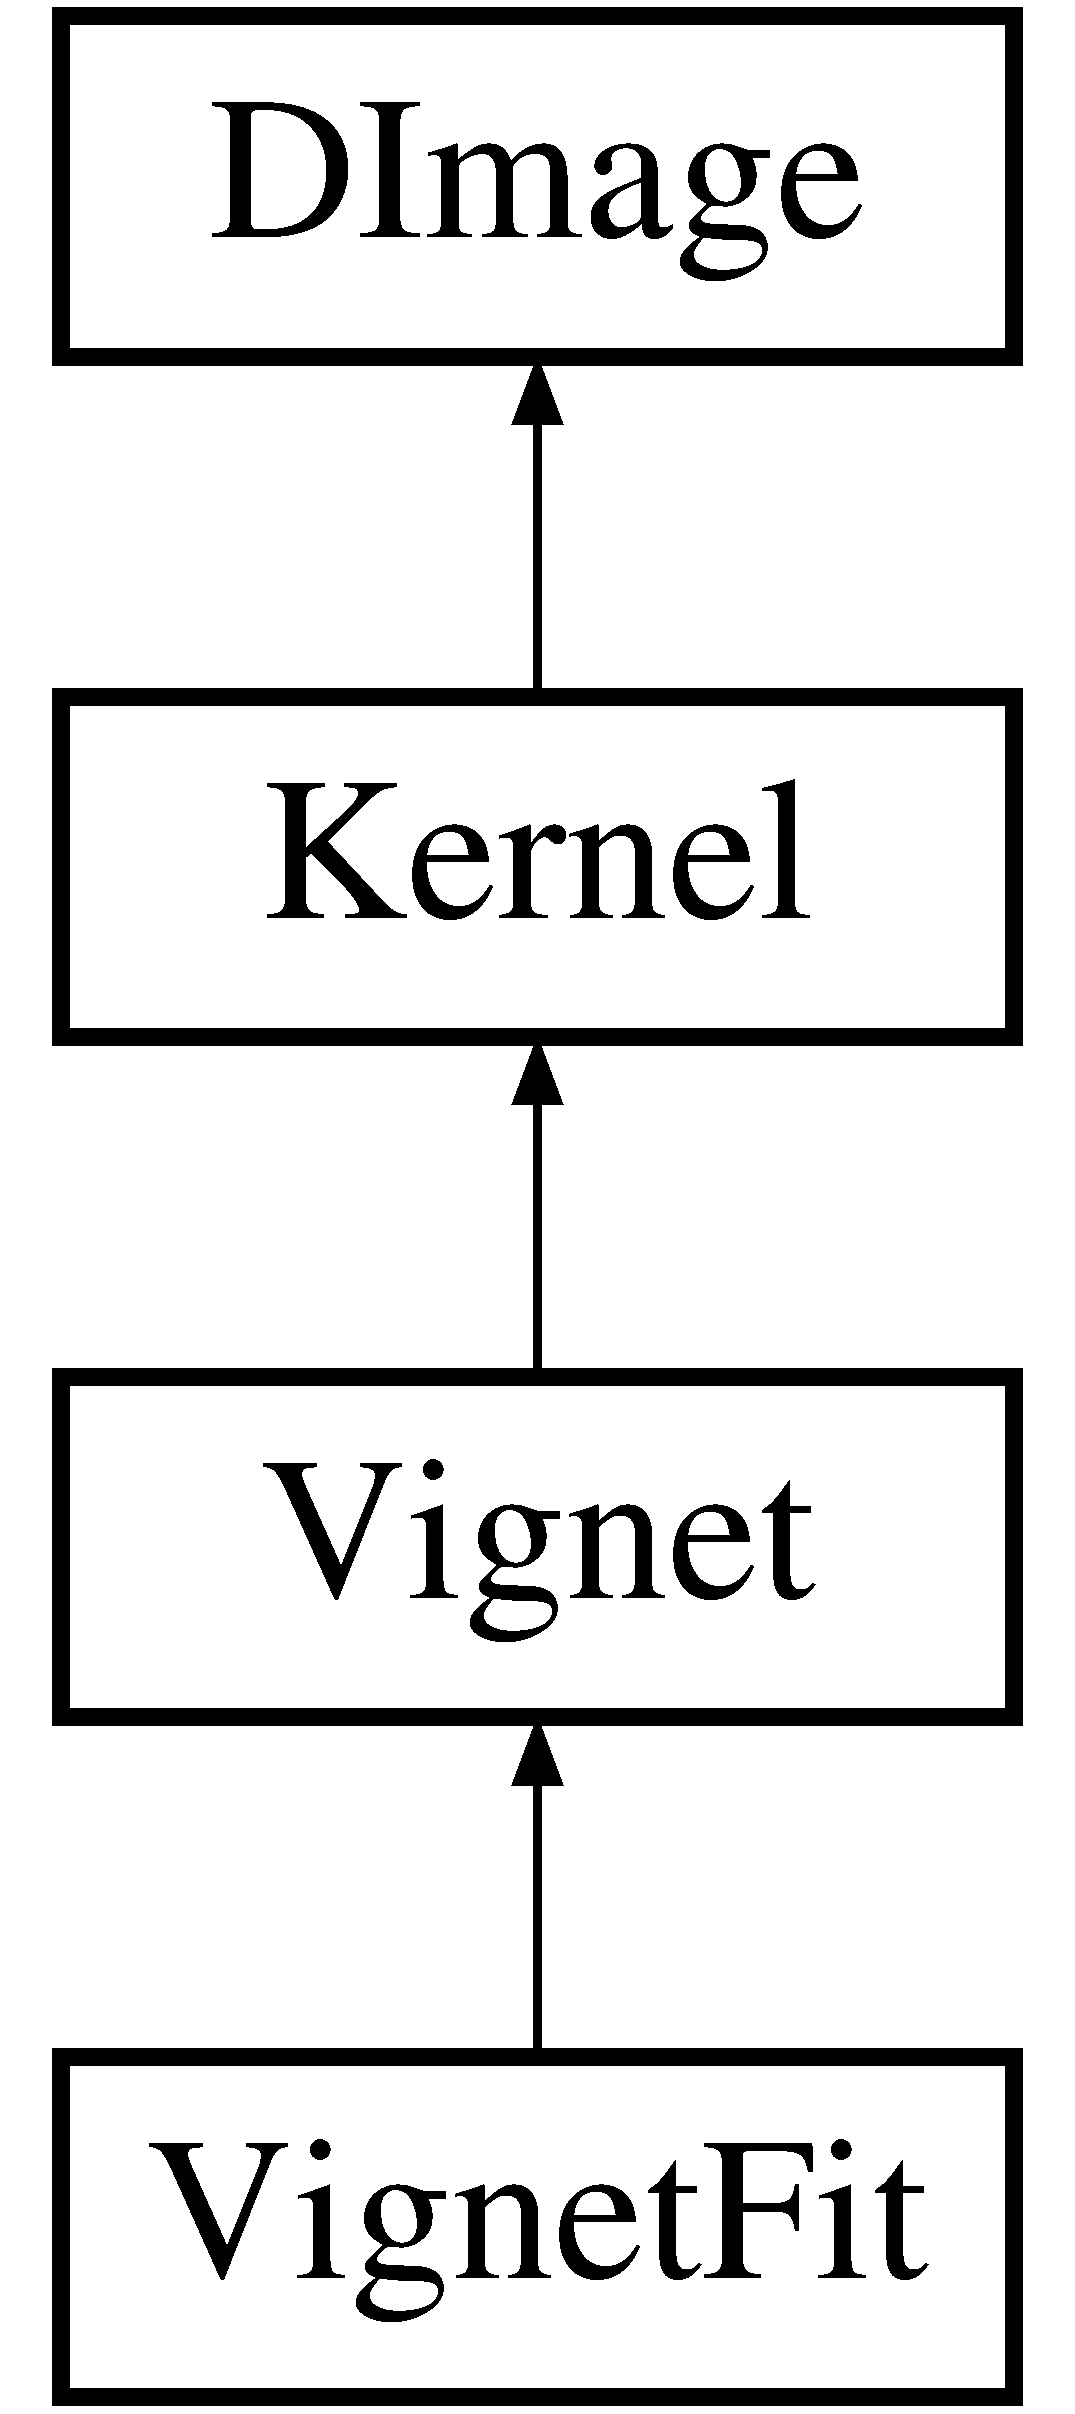
\includegraphics[height=4cm]{class_kernel}
\end{center}
\end{figure}
\subsubsection*{Public Methods}
\begin{CompactItemize}
\item 
\index{Kernel@{Kernel}!Kernel@{Kernel}}\index{Kernel@{Kernel}!Kernel@{Kernel}}
{\bf Kernel} (const int HSize)\label{class_kernel_a0}

\begin{CompactList}\small\item\em construtor for a square kernel of half size Hsize.\item\end{CompactList}\item 
\index{Kernel@{Kernel}!Kernel@{Kernel}}\index{Kernel@{Kernel}!Kernel@{Kernel}}
{\bf Kernel} (const int HSize\-X, const int HSize\-Y)\label{class_kernel_a1}

\begin{CompactList}\small\item\em construtor for a rectangle kernel of half sizes Hsize\-X and Hsize\-Y.\item\end{CompactList}\item 
\index{Kernel@{Kernel}!Kernel@{Kernel}}\index{Kernel@{Kernel}!Kernel@{Kernel}}
{\bf Kernel} (const {\bf DImage} \&Dim)\label{class_kernel_a2}

\item 
\index{Kernel@{Kernel}!Kernel@{Kernel}}\index{Kernel@{Kernel}!Kernel@{Kernel}}
{\bf Kernel} (const string \&Fits\-Name)\label{class_kernel_a3}

\item 
\index{Kernel@{Kernel}!Kernel@{Kernel}}\index{Kernel@{Kernel}!Kernel@{Kernel}}
{\bf Kernel} (const Kernel \&K, int Band\-X, int Band\-Y)\label{class_kernel_a4}

\begin{CompactList}\small\item\em builds a bigger kernel than a given one, and sets extra pixels in the surrounding band to zero.\item\end{CompactList}\item 
\index{Kernel@{Kernel}!Kernel@{Kernel}}\index{Kernel@{Kernel}!Kernel@{Kernel}}
{\bf Kernel} (const Kernel \&Other)\label{class_kernel_a5}

\item 
\index{Kernel@{Kernel}!Kernel@{Kernel}}\index{Kernel@{Kernel}!Kernel@{Kernel}}
{\bf Kernel} ()\label{class_kernel_a6}

\item 
\index{operator=@{operator=}!Kernel@{Kernel}}\index{Kernel@{Kernel}!operator=@{operator=}}
Kernel\& {\bf operator=} (const Kernel \&Right)\label{class_kernel_a7}

\item 
\index{readFits@{readFits}!Kernel@{Kernel}}\index{Kernel@{Kernel}!readFits@{read\-Fits}}
void {\bf read\-Fits} (const string \&Fits\-Name)\label{class_kernel_a8}

\begin{CompactList}\small\item\em write and read the {\bf DImage} {\rm (p.\,\pageref{class_dimage})} as a FITS array.\item\end{CompactList}\item 
\index{IsDirac@{IsDirac}!Kernel@{Kernel}}\index{Kernel@{Kernel}!IsDirac@{Is\-Dirac}}
bool {\bf Is\-Dirac} () const\label{class_kernel_a9}

\item 
\index{HSizeX@{HSizeX}!Kernel@{Kernel}}\index{Kernel@{Kernel}!HSizeX@{HSize\-X}}
int {\bf HSize\-X} () const\label{class_kernel_a10}

\begin{CompactList}\small\item\em half the size in x direction.\item\end{CompactList}\item 
\index{HSizeY@{HSizeY}!Kernel@{Kernel}}\index{Kernel@{Kernel}!HSizeY@{HSize\-Y}}
int {\bf HSize\-Y} () const\label{class_kernel_a11}

\begin{CompactList}\small\item\em half the size in y direction.\item\end{CompactList}\item 
\index{KeepCircleOnly@{KeepCircleOnly}!Kernel@{Kernel}}\index{Kernel@{Kernel}!KeepCircleOnly@{Keep\-Circle\-Only}}
void {\bf Keep\-Circle\-Only} (const double \&radius)\label{class_kernel_a12}

\begin{CompactList}\small\item\em zero out outside a given radius.\item\end{CompactList}\item 
\index{FillWithGaussian@{FillWithGaussian}!Kernel@{Kernel}}\index{Kernel@{Kernel}!FillWithGaussian@{Fill\-With\-Gaussian}}
void {\bf Fill\-With\-Gaussian} (const double \&xc, const double \&yc, const double \&sigmax, const double \&sigmay, const double \&rho=0)\label{class_kernel_a13}

\begin{CompactList}\small\item\em fills the kernel array with a 2d normalized gaussian (xc and yc are in kernel coordinates).\item\end{CompactList}\item 
\index{dump@{dump}!Kernel@{Kernel}}\index{Kernel@{Kernel}!dump@{dump}}
void {\bf dump} () const\label{class_kernel_a14}

\begin{CompactList}\small\item\em prints all kernel values.\item\end{CompactList}\item 
\index{bias@{bias}!Kernel@{Kernel}}\index{Kernel@{Kernel}!bias@{bias}}
void {\bf bias} (double \&x, double \&y) const\label{class_kernel_a15}

\begin{CompactList}\small\item\em computes mean of the kernel on (x,y).\item\end{CompactList}\item 
\index{dump_info@{dump\_\-info}!Kernel@{Kernel}}\index{Kernel@{Kernel}!dump_info@{dump\_\-info}}
void {\bf dump\_\-info} (ostream \&stream=cout) const\label{class_kernel_a16}

\begin{CompactList}\small\item\em prints bias and moments of the kernel.\item\end{CompactList}\item 
\index{moments@{moments}!Kernel@{Kernel}}\index{Kernel@{Kernel}!moments@{moments}}
void {\bf moments} (double \&vx, double \&vy, double \&vxy) const\label{class_kernel_a17}

\begin{CompactList}\small\item\em computes x and y first order moments of the kernel ($\backslash$sigma\_\-x, $\backslash$sigma\_\-y, $\backslash$rho\_\-\{xy\}).\item\end{CompactList}\item 
\index{IsEmpty@{IsEmpty}!Kernel@{Kernel}}\index{Kernel@{Kernel}!IsEmpty@{Is\-Empty}}
bool {\bf Is\-Empty} () const\label{class_kernel_a18}

\item 
\index{MaxPixel@{MaxPixel}!Kernel@{Kernel}}\index{Kernel@{Kernel}!MaxPixel@{Max\-Pixel}}
void {\bf Max\-Pixel} (double \&xmax, double \&ymax)\label{class_kernel_a19}

\item 
\index{MinPixel@{MinPixel}!Kernel@{Kernel}}\index{Kernel@{Kernel}!MinPixel@{Min\-Pixel}}
void {\bf Min\-Pixel} (double \&xmin, double \&ymin)\label{class_kernel_a20}

\end{CompactItemize}
\subsubsection*{Protected Attributes}
\begin{CompactItemize}
\item 
\index{hSizeX@{hSizeX}!Kernel@{Kernel}}\index{Kernel@{Kernel}!hSizeX@{h\-Size\-X}}
int {\bf h\-Size\-X}\label{class_kernel_n0}

\item 
\index{hSizeY@{hSizeY}!Kernel@{Kernel}}\index{Kernel@{Kernel}!hSizeY@{h\-Size\-Y}}
int {\bf h\-Size\-Y}\label{class_kernel_n1}

\end{CompactItemize}


\subsubsection{Detailed Description}
An odd size {\bf DImage} {\rm (p.\,\pageref{class_dimage})} addressed with (0,0) at center allows quick computation of convolution like operations.



The documentation for this class was generated from the following file:\begin{CompactItemize}
\item 
{\bf dimage.h}\end{CompactItemize}
